\section{CMOS}
\begin{center}
    \begin{minipage}{0.45\linewidth}
        \subsubsection{NMOS}
        \begin{center}
            \begin{adjustbox}{height = 30mm}
                \begin{circuitikz}[european]
                    \node[circ, label=90:{\small $V_{DD} = 0.8 \si{\volt}$}](origin) at (0,0) {};
                    \node[thick, nmos, anchor=D] (nmos1) at(0, -2) {};
                    \draw[thick] 
                        (origin)
                        to[R=$R$] (0,-1.8) node[circ] (ybase) {}
                        to[] (0, -2);


                    \draw[thick] (nmos1.S) -- (0, -3.7) coordinate(gnd);
        
                    \node[pin=90:G] at (nmos1.G) {};
                    \node[pin=300:D] at (nmos1.D) {};
                    \node[pin=30:S] at (nmos1.S) {};
        
                    \path[draw] (ybase) --++(right:5mm) node[point, label=0:Y] {};
                    \path[draw, very thick] (-0.25, -3.7) -- (gnd) -- (0.25, -3.7);
                \end{circuitikz}
            \end{adjustbox}
        \end{center}
        \begin{center}
            \begin{tabular}{c|c|c}
                G & Schalter & Y\\
                \hline
                0 & offen & 1\\
                1 & zu & 0
            \end{tabular}
        \end{center}
    \end{minipage}
    \hfill
    \begin{minipage}{0.45\linewidth}
        \subsubsection{PMOS}
        \begin{center}
            \begin{adjustbox}{height = 30mm}
                \begin{circuitikz}[european]
                    \coordinate (gnd) at (0, -4);
                    \node[circ, label=90:{\small $V_{DD} = 0.8 \si{\volt}$}] (vdd) at (0,0) {};
                    \node[pmos, thick] (pmos) at (0, -1){};

                    \draw[thick] (gnd) 
                        to[R=$R$] (0, -2) 
                        -- (0, -2) node[circ] (ybase) {}
                        -- (pmos.D);
                    
                    \draw[thick] (pmos.S) -- (vdd);

                    \node[pin=90:G] at (pmos.G) {};
                    \node[pin=30:D] at (pmos.D) {};
                    \node[pin=300:S] at (pmos.S) {};
        
                    \path[draw] (ybase) --++(right:5mm) node[point, label=0:Y] {};
                    \path[draw, very thick] (-0.25, -4) -- (gnd) -- (0.25, -4);
                \end{circuitikz}
            \end{adjustbox}
        \end{center}
        \begin{center}
            \begin{tabular}{c|c|c}
                G & Schalter & Y\\
                \hline
                0 & zu & 1\\
                1 & offen & 0
            \end{tabular}
        \end{center}
    \end{minipage}
\end{center}

\subsection{Konstruktion von CMOS-Gates}
Regeln für CMOS-Schaltungen
\begin{enumerate}
    \item CMOS-Gates bestehen aus gleich vielen NMOS und PMOS.
    \item $m$ Eingänge: $m$ NMOS und $m$ PMOS.
    \item NMOS in Serie $\rightarrow$ PMOS parallel
    \item NMOS parallel $\rightarrow$ PMOS Serie
\end{enumerate}

\subsubsection{Allg. Aufbau CMOS}
\begin{center}
    \begin{minipage}{0.3\linewidth}

        \begin{center}
            \begin{tikzpicture}
                \node[circ] at (0,0) (origin) {};
                \node[draw, dotted](pmos) at(0,-0.5) {PMOS};
                \node[draw, dotted](nmos) at (0, -1.5) {NMOS};
                \coordinate(gnd) at (0, -2){};
                \draw[] (origin) -- (pmos)
                    (pmos) -- (nmos)
                    (nmos) -- (gnd);
                \path[draw] (0,-1) --++(right:5mm) node[fill = white] {Y};
                \path[draw, thick] (-0.25, -2) -- (gnd) -- (0.25, -2);
            \end{tikzpicture}
        \end{center}
    \end{minipage}
    \begin{minipage}{0.55\linewidth}
        \begin{flushleft}
            \begin{tabular}{l l}
                Pull-u\textcolor{red}{p}: & \textcolor{red}{P}MOS\\
                Pull-dow\textcolor{red}{n}: & \textcolor{red}{N}MOS\\
            \end{tabular}
        \end{flushleft}
        Pfade sind komplementär (\textbf{Serie $\Leftrightarrow$ Parallel})
    \end{minipage}
\end{center}
\subsubsection{Umwandlung Pull-up zu Pull-down}
\begin{enumerate}
    \item Teilbereiche (Blöcke) identifizieren.
    \item Schritt 1 wiederholen, bis nur noch einzelne Transistoren vorkommen. 
    \item Falls Pull-down:
    \begin{itemize}
        \item Von GND aus mit äusserstem Block beginnen.
        \item PMOS $\rightarrow$ NMOS
    \end{itemize}
    \item Falls Pull-up:
    \begin{itemize}
        \item Von $V_{DD}$ aus mit äusserstem Block beginnen.
        \item NMOS $\rightarrow$ PMOS.
    \end{itemize}
\end{enumerate}
% 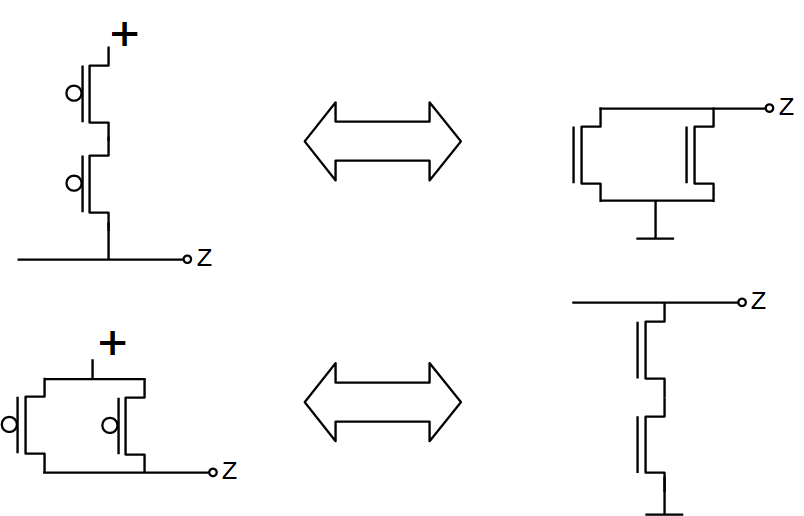
\includegraphics[width = 30mm]{images/pnmosDetConv.png}
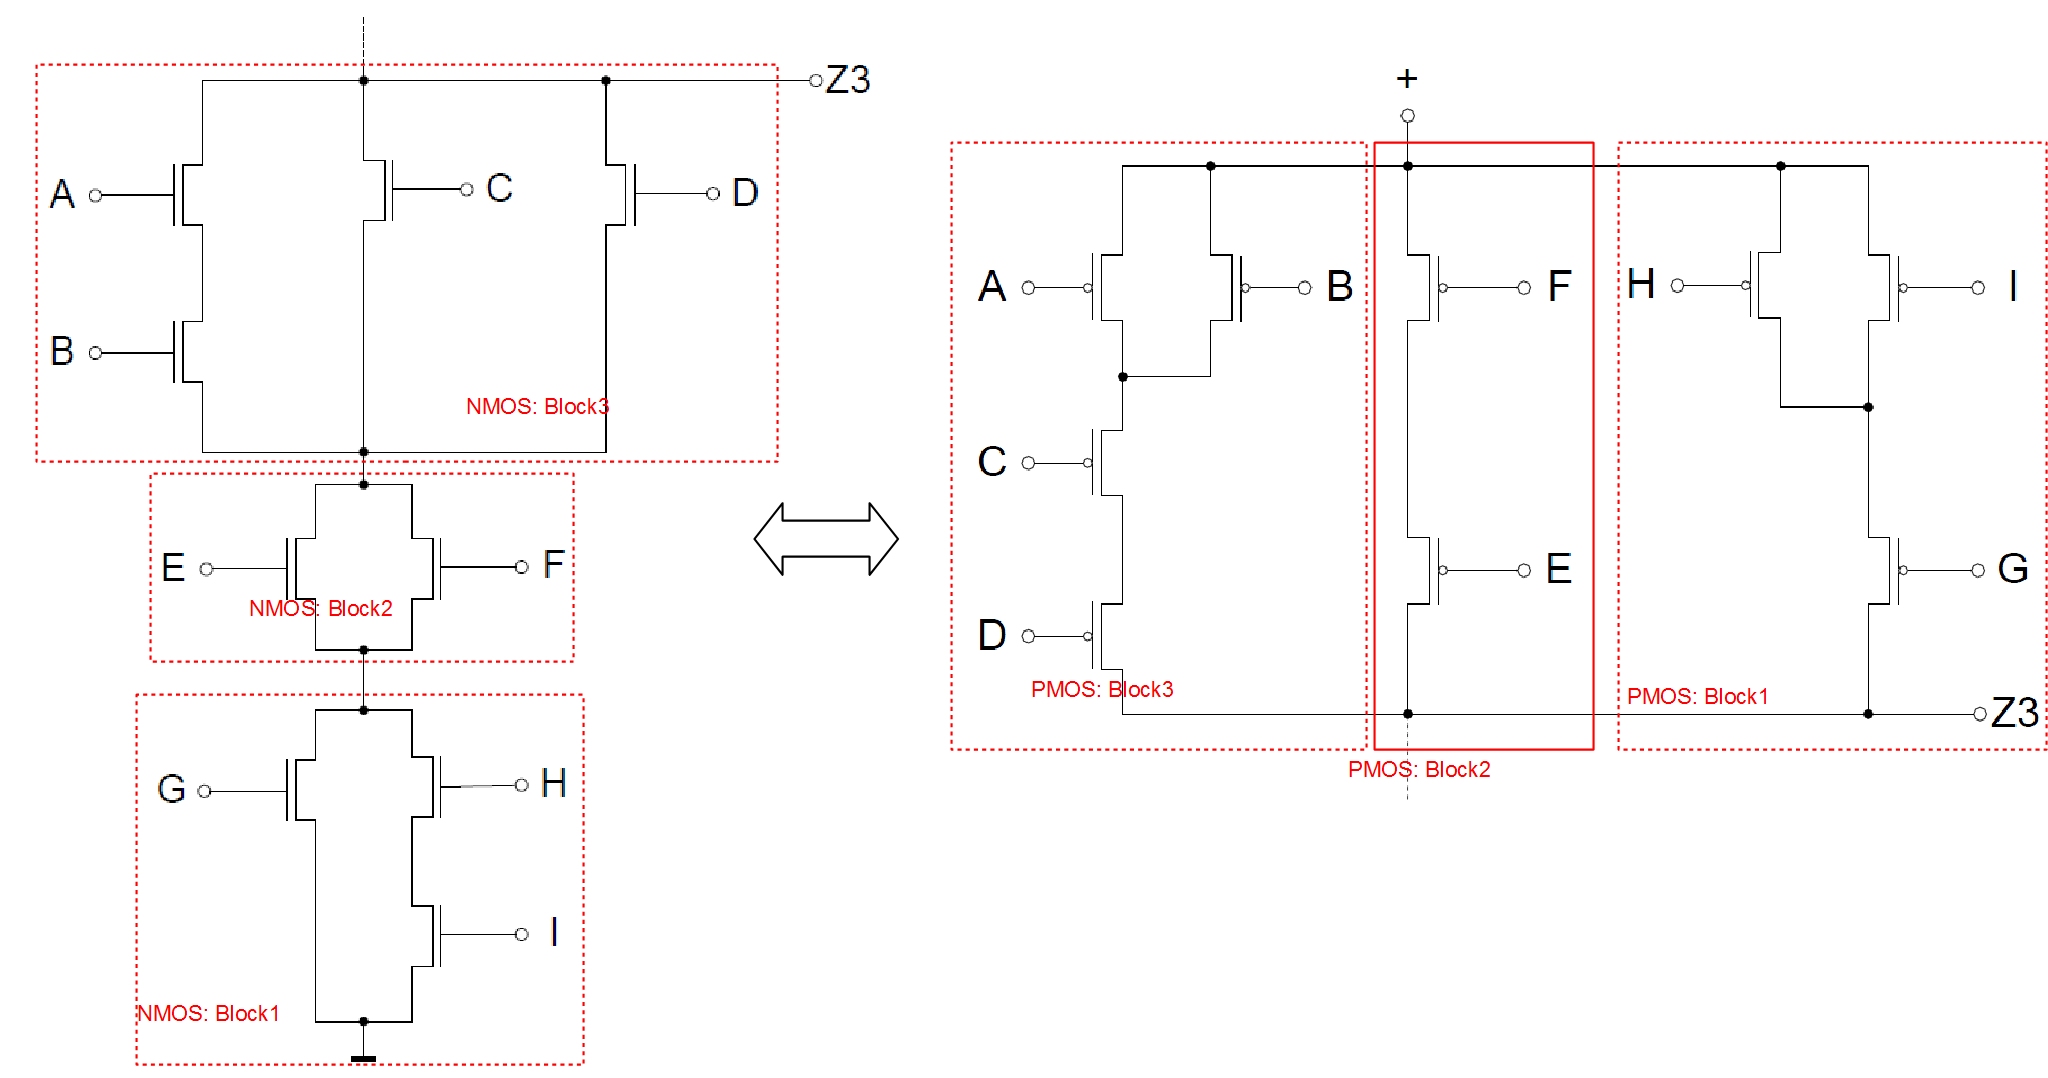
\includegraphics[width = 68mm]{images/pnmosconv.png}
\subsubsection{Funktionsgleichung}
\begin{flushleft}
    \small
    \begin{tabular}{l|l l}
        parallel: $\lor$ & Pull-Up: $y=1$ & $\text{alle I}: 0 \rightarrow \text{I invert.}$\\
        Serie: $\land$ & Pull-Down: $y=0$ & $\text{alle I}: 1 \rightarrow \text{Gl. invert.}$\\
    \end{tabular}
\end{flushleft}